\section{Estado del arte}

Como decíamos anteriormente, en los últimos años, la investigación en visión artificial se ha convertido en sinónimo de deep learning, siendo uno de los dominios donde más progreso se está logrando. Las principales áreas de investigación son segmentación semántica, clasificación de imágenes y detección de objetos. Recientemente se han empezado empezado a popularizar las técnicas de generación de imágenes, por ejemplo caras aleatorias o también la de sustituir la cara de una persona en un vídeo por otra, técnica que es conocida como \textit{deepfake}.

Esta última técnica está sujeta a gran controversia por su fácil uso como herramienta de desinformación y propaganda dada la dificultad que supone distinguir un vídeo manipulado de uno real. Esta preocupación por el uso de \textit{deepfakes} para deslegitimar a adversarios políticos ha llevado a Microsoft a presentar un sistema detector de vídeos que emplean esta técnica \cite{deepFake}.

Las tareas de reconocimiento de objetos y segmentación se han visto beneficiadas de la existencia de grandes datasets como PASCAL VOC, ImageNet o COCO. El último de ellos fue propuesto por Microsoft para tareas de detección de objetos, segmentación y razonamiento contextual. Contiene 328 mil imágenes, 2.5 millones de instancias anotadas y 91 clases. El trabajo que mayor porcentaje de éxito ha tenido sobre este dataset ha sido el realizado por \citet{Tan_2020}, con un box AP (precisión media de las cajas del detector) de $55.1\%$ y un AP50 (más del 50\% de intersección entre la caja etiquetada y la que detecta el modelo) de $74.3\%$. Este es un gran resultado teniendo en cuenta la dificultad del dataset, aunque también puede verse que queda aún un largo camino por recorrer.

Si bien Google Maps ya venía ofreciendo un servicio de modelos 3D de mapas en base a imágenes de satélite, el nuevo simulador de vuelo lanzado por Microsoft (\textit{Microsoft Flight Simulator}) ofrece un mapa a escala real completamente generado utilizando dicha técnica, siendo así el primer videojuego que emplea \textit{deep learning} a esta escala. Utilizando datos satelitales y fotogrametría, el juego genera ciudades reales con todos sus monumentos y modela la meteorología en tiempo real. El mapa generado ocupa 2 petabytes y se va cargando al ordenador por \textit{streaming}.

\begin{figure}
    \centering
    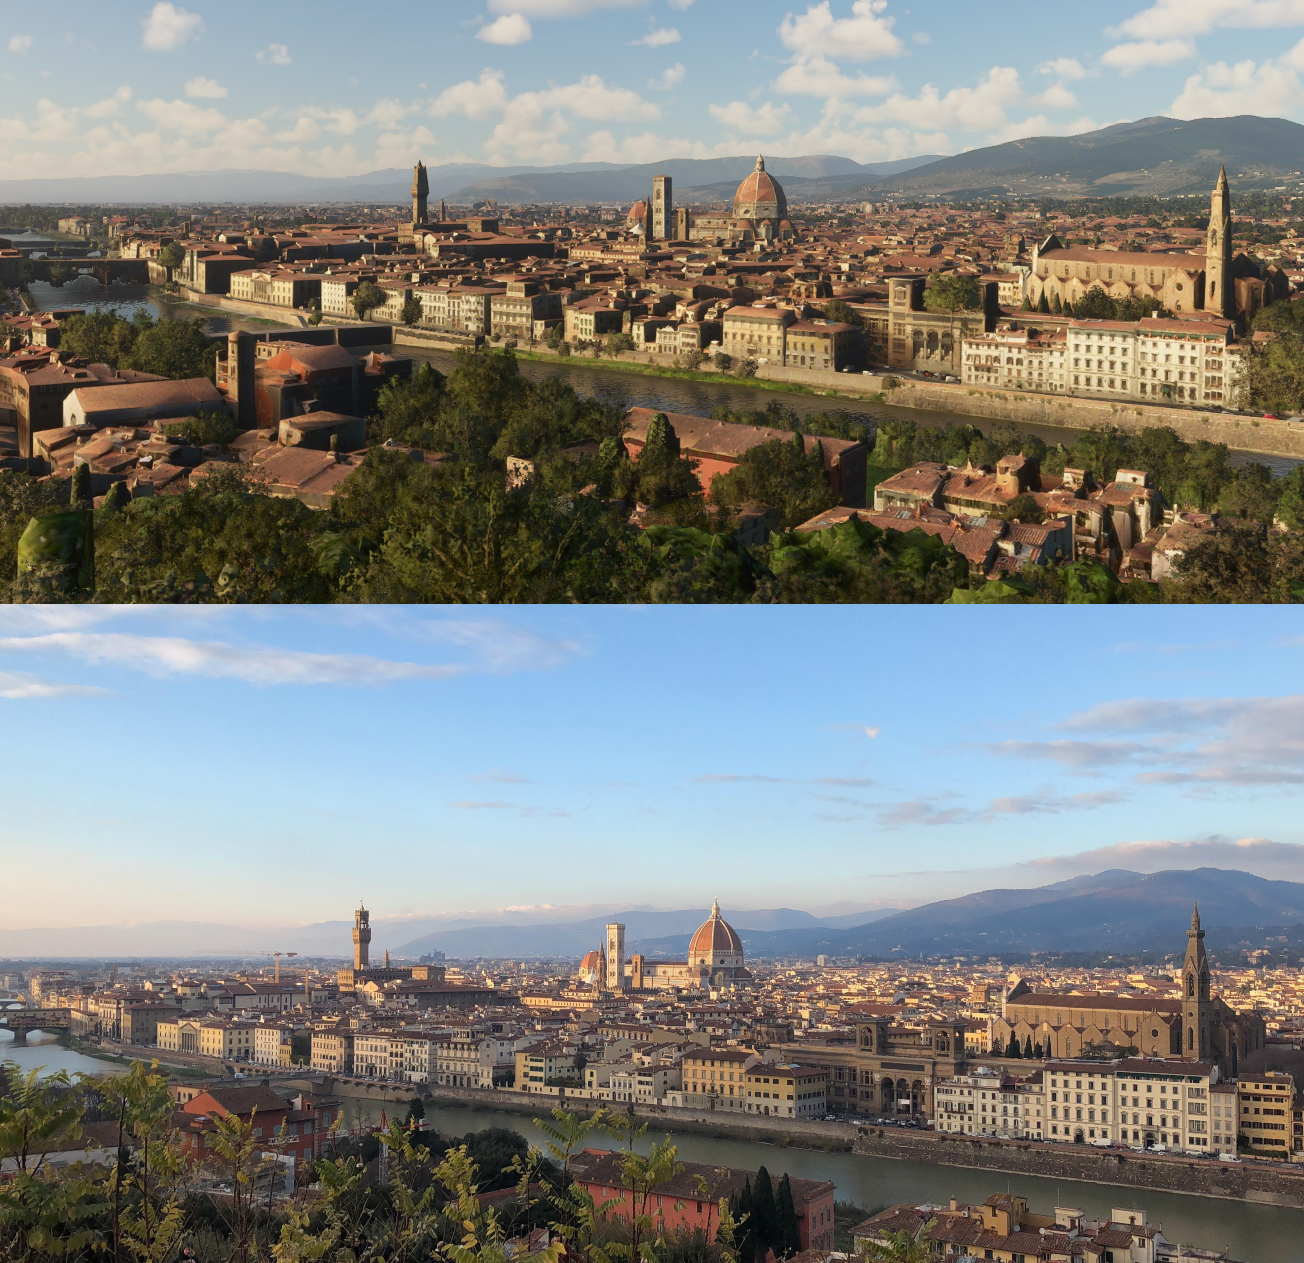
\includegraphics[width=0.6\textwidth]{images/fls2020.png}
    \caption{Imagen comparativa entre la Florencia generada por Microsoft Flight Simulator (arriba) y la Florencia real (abajo) (Fuente: \href{https://www.reddit.com/r/MicrosoftFlightSim/comments/ic559l/photo_of_florence_from_the_piazzale_michelangelo/}{Reddit}).}
    \label{fig:fs2020}
\end{figure}

También en la industria del videojuego, la demanda por cada vez mayores resoluciones y gráficos más realistas hace que, en algunos casos, los modelos más modestos de tarjetas gráficas tengan problemas de rendimiento. Para mejorar este problema, Nvidia publicó en 2018 junto con su serie RTX 20 una tecnología denominada DLSS (\textit{Deep Learning Super Sampling}). Esta tecnología consiste en renderizar imágenes a resoluciones inferiores (por ejemplo, 1080p) y sobremuestrearlas a otras resoluciones más altas (por ejemplo, 4k) utilizando una red neuronal que produce la imagen sobremuestreada por medio de una predicción de los píxels ``que faltan''.

\subsection{Visión artificial en los deportes}
Una vez revisadas las aplicaciones actuales de visión artificial en general, vamos a centrarnos en aquellas aplicaciones del campo que nos atañe, el deporte.

Quizá una de las aplicaciones más famosas de la visión por computador a los deportes sea el ojo de halcón, desarrollado por la compañía Hawk-Eye. Este sistema se viene utilizando en gran diversidad de deportes: tenis, cricket, rugby, volleyball, fútbol... La primera vez que se utiliza el ojo de halcón fue en 2001, en retransmisiones de cricket, donde se utilizaba para seguir las trayectorias de las bolas.

La aplicación más conocida de esta tecnología es, seguramente, en el tenis. El sistema se utiliza por primera vez en un torneo de élite en 2006 en la copa Hopman, y el primer grand-slam en hacer uso de él fue el US Open de ese mismo año. Si bien con los años se ha ido considerando parte del propio deporte, durante los inicios de su utilización fue fruto de controversias por algunos errores del sistema.

En fútbol, tras controversias como un \textit{gol fantasma} en el mundial de 2010 que acabó provocando la eliminación de Inglaterra ante Alemania (y otras controversias en mundiales anteriores), se implementó en el mundial de clubes de 2012 la tecnología llamada \textit{goal-line technology}, desarrollada por la misma compañía que el ojo de halcón del tenis. El objetivo de este sistema era el de decir si un balón había pasado la línea de gol o no en jugadas en que no estuviera claro. 

El funcionamiento del sistema es similar en todos los deportes que lo utilizan: consiste en una serie de cámaras (10, en tenis) que toman imágenes de distintos ángulos del área de juego, y usando principios de triangulación, se calcula la localización actual de la pelota y se ``predice'' su posición siguiente \cite{wiki:hawk}.

Otra aplicación de la tecnología en el fútbol es el sistema conocido como VAR, que se ha puesto en marcha desde el mundial de 2018. Este es en gran parte operado por un árbitro en una cabina con varios ángulos de cámara, pero también se incluye una tecnología para trazar las líneas del fuera de juego de forma automática, respetando la perspectiva de la cámara que se usa.


\begin{figure}
    \centering
    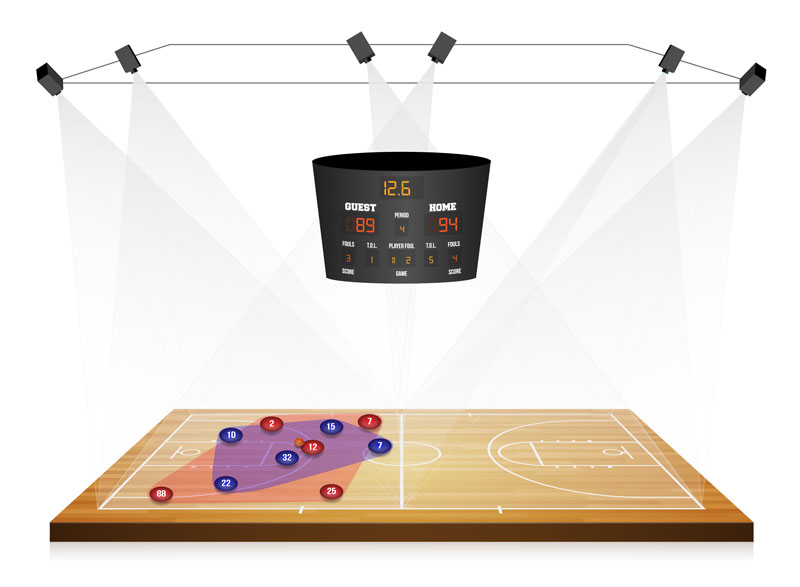
\includegraphics[width=0.6\textwidth]{images/sportVU}
    \caption{Diagrama informativo de la instalación de SportVU en un campo de baloncesto \cite{tfg}.}
    \label{fig:sportVU}
\end{figure}

Existen otras soluciones que permiten recabar estadísticas del partido, como es el caso de SportVU o Kinexon. En baloncesto (figura \ref{fig:sportVU}), la instalación consiste en un sistema de 3 a 6 cámaras, que recopilan datos de jugadores y balón 25 veces por segundo y calcula estadísticas tales como distancia viajada, velocidad media, velocidad máxima, mapas de calor, posesión, distancia y precisión de los tiros. Sin embargo, está disponible para más deportes: fútbol, fútbol americano, béisbol, hockey sobre hielo y rugby. En la NBA esta tecnología se viene implantando desde la temporada 2010-11. En la temporada 2016-17, cuando el sistema se utilizaba en todos los equipos de la NBA, la liga extendió el contrato con SportVU e hizo disponibles las estadísticas a medios de comunicación tales como ESPN o TNT.

Existen también otros sistemas utilizados para la ayuda en la retransmisión televisiva. Es el caso del sistema desarrollado por Intel, denominado Intel 360 Replay. Este sistema provee de repeticiones en 3D de jugadas, utilizando 38 cámaras con resolución 5K. Se viene utilizando desde hace unos años en la NBA y la MLB y más recientemente en fútbol. Uno de los primeros grandes partidos en utilizar el sistema fue el clásico de la temporada 2016-17.

En deportes con un fondo uniforme, como los que emplean pistas de césped, se puede utilizar este fondo como un croma para hacer dibujos en el campo de juego, como escudos o trayectorias de jugadores. Esta técnica ha sido empleada durante esta temporada para sustituir las gradas vacías (por las normativas sanitarias) por fotos de público.

Un área de investigación actual es la automatización de la realización de las retransmisiones deportivas. Esta es una tarea complicada ya que requiere de dos tareas: el seguimiento de la acción y la búsqueda del mejor plano para visualizar esta. La tecnología esta lejos de ser una realidad, pero existe un acercamiento posible como que un realizador maneje una cámara principal que es capaz de determinar la posición a la que apunta y le manda dicha posición a una serie de cámaras que enfocan al mismo lugar \cite{book:cvInSports}.

Utilizando deep learning, se han publicado trabajos como el de \citet{art:DeepBall}, en el que se desarrolló un detector especializado en balones, utilizando una red completamente convolucional (figura \ref{fig:deepball}) y que produce un mapa de confianza con las posibles posiciones del balón. Este modelo era superior a otros dos anteriormente propuestos, logrando una precisión media de $87.7\%$, utilizando \textit{data augmentation}. Un problema que tenía el modelo eran las oclusiones de balón así como objetos de pequeño tamaño y de color similar al balón que engañaban al modelo (figura \ref{fig:deepballerror}).

\begin{figure}
    \centering
    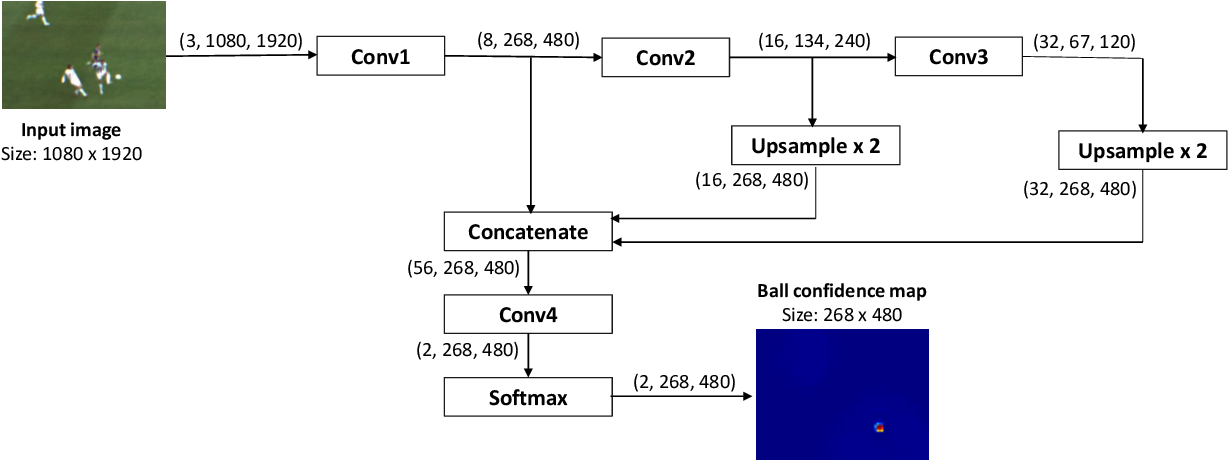
\includegraphics[width=0.7\textwidth]{images/deepball}
    \caption{Visualización de la arquitectura propuesta en DeepBall \cite{art:DeepBall}.}
    \label{fig:deepball}
\end{figure}


\begin{figure}
    \centering
    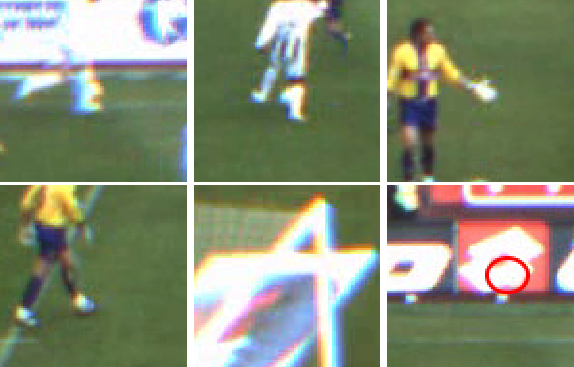
\includegraphics[width=0.4\textwidth]{images/errorDeepball.png}
    \caption{Algunos de los errores de detección del modelo DeepBall \cite{art:DeepBall}.}
    \label{fig:deepballerror}
\end{figure}

Una aplicación reciente a deportes (aunque menos convencionales), que hereda el espíritu de Deep Blue, son las tecnologías de DeepMind, empresa que desarrolla sistemas de redes neuronales para jugar a juegos tales como Go, Backgammon o Starcraft. AlphaGo fue un sistema creado con el objetivo de vencer al campeón mundial de Go, Ke Jie. En 2017, el sistema consiguió vencerle. El sucesor de AlphaGo, AlphaZero \cite{AlphaZero}, está actualmente considerado el mejor jugador del mundo de Go.

Una trabajo cercano al nuestro es el de \citet{volleyDeep}. En él, el autor se enfrentaba a un problema parecido al que nos hemos propuesto en este trabajo, con la diferencia de que en este caso se utilizaba una cámara a nivel de grada y no desde arriba. Para salvar los fallos de detección relativamente frecuentes del modelo, el autor utilizó un análisis de trayectorias de las formas que se detectaban en la escena, donde aquellas más parecidas a una parábola eran identificadas como balón. Este análisis se plantea como un tipo de consistencia temporal ya que la detección desde cero no era factible en el modelo logrado.

\newpage